\documentclass[a4paper,12pt]{article}% Seu arquivo fonte precisa conter
\usepackage[brazil]{babel} % estas quatro linhas
\usepackage[utf8]{inputenc} % aléem do comando \end{document}

\usepackage{listings}
\usepackage{graphicx}
\usepackage{url}

\begin{document} % no fim.



\begin{titlepage}

\newcommand{\HRule}{\rule{\linewidth}{0.5mm}} % Defines a new command for the horizontal lines, change thickness here

\center % Center everything on the page
 
%----------------------------------------------------------------------------------------
%	HEADING SECTIONS
%----------------------------------------------------------------------------------------

\textsc{\LARGE Universidade Federal\\do Espírito Santo}\\[1.5cm] % Name of your university/college
\textsc{\Large Centro Tecnológico}\\[0.5cm] % Major heading such as course name
\textsc{\large Departamento de Informática}\\[0.5cm] % Minor heading such as course title

%----------------------------------------------------------------------------------------
%	TITLE SECTION
%----------------------------------------------------------------------------------------

\HRule \\[0.4cm]
{ \huge \bfseries Interpretador de Sistemas de Lindenmayer}\\[0.4cm] % Title of your document
\HRule \\[1.5cm]

%----------------------------------------------------------------------------------------
%	AUTHOR SECTION
%----------------------------------------------------------------------------------------

\begin{minipage}{0.4\textwidth}
\begin{flushleft} \large
\emph{Autor:}\\
Vinicius \textsc{Arruda} % Your name
\end{flushleft}
\end{minipage}
~
\begin{minipage}{0.4\textwidth}
\begin{flushright} \large
\emph{Professor:} \\
Thomas W. \textsc{Rauber} % Supervisor's Name
\end{flushright}
\end{minipage}\\[2cm]

% If you don't want a supervisor, uncomment the two lines below and remove the section above
%\Large \emph{Author:}\\
%John \textsc{Smith}\\[3cm] % Your name

%----------------------------------------------------------------------------------------
%	DATE SECTION
%----------------------------------------------------------------------------------------

{\large \today}\\[2cm] % Date, change the \today to a set date if you want to be precise

%----------------------------------------------------------------------------------------
%	LOGO SECTION
%----------------------------------------------------------------------------------------


\includegraphics[width=58mm]{LogoUfes.png}\\[1cm] % Include a department/university logo - this will require the graphicx package

%----------------------------------------------------------------------------------------

\vfill % Fill the rest of the page with whitespace

\end{titlepage}





\begin{abstract}
Trabalho da disciplina de Estrutura de Dados I, que consiste no desenvolvimento 
de um interpretador de sistemas de Lindenmayer, utilizando conceitos de estrutura 
de dados e tipos abstratos de dados para a elaboração do trabalho.
\end{abstract}

\begin{figure}[hb!]
\centering
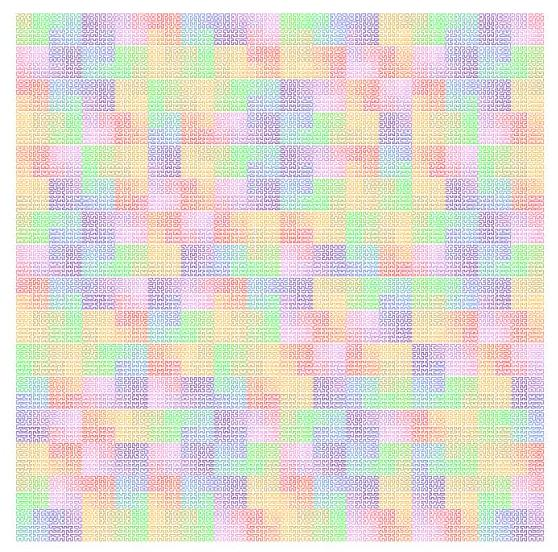
\includegraphics[width=140mm]{hilbert.jpg}
\caption{Hilbert.}
\end{figure}
\hspace{1.5em}Imagem gerada a partir do interpretador desenvolvido.
\newpage






\section{Introdução} % Este comando faz o tíıtulo da seção.
%INTRODUÇÃO

% compilação foi utilizado o compilador GCC versão 4.7.2 em uma máquina a

\hspace{1.5em}Ao implementar um sistema, frequentemente programadores se deparam com o uso de 
estruturas de dados que na maioria das vezes são estáticas como os vetores e matrizes 
por exemplo. Porém, ao implementar um sistema mais complexo, surge a necessidade de 
se trabalhar com tipos dinâmicos e mais específicos para aquele problema.
	
O ideal é abstrair este tipo para que torne a vida do programador mais fácil. Essa 
é a idéia do tipo abstrato de dados, comumente conhecido como TAD.

O sistema aqui implementado, faz o uso de vários TADs para abstrair a manipulação dos dados 
do próprio programador, fazendo com que o desenvolvimento do sistema seja feito em camadas, 
de maneira mais organizada.	

Para a implementação dos TADs, foram utilizados estruturas de dados estáticas, alocação dinâmica de memória, 
tipo genérico, funções de callback e os conceitos de lista encadeada, árvore e pilha.

%OBJETIVO:
\section{Objetivo}
\hspace{1.5em}Aplicar o conhecimento adquirido na disciplina de Estruturas de Dados I para representar
e manipular informações estruturada por linguagem de programação de alto nível na elaboração 
de um interpretador de sistemas de Lindenmayer.

%FERRAMENTAS:
\section{Ferramentas}
\hspace{1.5em}O interpretador foi implementado na linguagem de programação C. Para a compilação foi 
utilizado o compilador GCC versão 4.7.2 em uma máquina com o sistema operacional Debian 
GNU/Linux 7.8 (wheezy).
O código foi escrito utilizando o editor de texto gedit versão 3.4.2.
Para a depuração do programa, foi utilizado a ferramenta Valgrind versão 3.7.0.


%METODOLOGIA:
\section{Metodologia}
\hspace{1.5em}O desenvolvimento do interpretador foi dividido em três etapas, que se basearam em construir o parser, 
a árvore de filhos variados para aplicar as regras e os comandos para as partes 2 e 3 do trabalho.

\subsection{O Parser}
	
\hspace{1.5em}A função do parser e de sua função auxiliar para a leitura do arquivo, consiste em interpretar do arquivo as 
informações para preencher as estruturas \emph{preamble} e \emph{productions} que armazenarão as informações necessárias 
para a geração do \emph{l-system}.
\newline
\newline
\hspace{1.5em}As estruturas \emph{preamble} e \emph{productions} possuem a seguinte forma:

\begin{verbatim}
typedef struct                typedef struct
{                             {                              
    int angle;                     char* axiom;
    long int order;                List* rules
    double rotate;            } Productions;      
} Preamble;                   
                             
\end{verbatim}

Onde \emph{List} é um tipo definido em:

\begin{verbatim}
struct list                     
{
    void* info;                 
    struct list* next;         
};

typedef struct list List;
\end{verbatim}

Que é a estrutura de uma lista genérica encadeada utilizada para manipular \emph{rules}, que 
é uma lista de regras onde cada elemento é definido por:

\begin{verbatim}
typedef struct                                     
{
    char p;                     
    char* s;                                     
} Rule;
\end{verbatim}

Onde \emph{p} é um símbolo único e \emph{s} uma string que seguem a igualdade \emph{p = s}.

Quando a função de leitura do arquivo \emph{getStrings} lê uma linha do arquivo, 
ela chama a função \emph{parser} para analisar esta linha.

Ao identificar uma palavra chave, uma função própria para manipular esta informação é chamada, preenchendo 
seu devido campo em \emph{preamble} e \emph{productions}.

Ao encontrar um símbolo, uma função para manipular as regras é chamada, encadeando uma nova regra \emph{Rule} 
na lista \emph{rules} da estrutura \emph{productions}.


\subsection{A árvore}

\hspace{1.5em}A implementação do TAD árvore consistiu, primeiramente, na representação da informação, que consiste em um 
nó \emph{Tree} que possui sua informação, um ponteiro para seu nó irmão, um ponteiro para seu primeiro filho e um ponteiro para 
seu último filho. 
\newline
\newline
A estrutura da árvore possue a seguinte forma: 

\begin{verbatim}
typedef struct tree                                     
{
    char info;                                  
    struct tree* firstChild;                   
    struct tree* lastChild;                    
    struct tree* next;                         
} Tree;
\end{verbatim}

O motivo de um ponteiro extra, apontando para o último filho, se dá para otimizar no encadeamento dos nós, pois pela estrutura 
do interpretador, a informação deve ser encadeada na árvore da esquerda para a direita, tendo sempre que percorrer até o final da lista 
para encadear no último nó. Uma outra solução seria armazenar um ponteiro temporário para o final da lista a medida que as regras eram 
interpretadas e encadeadas, porém como o trabalho foi desenvolvido em camadas, foi preferido criar as estruturas de dados abstratas e ir 
trabalhando com essas abstrações.

A Figura \ref{fig:Tree} mostra um diagrama do TAD árvore elaborado.
\newline
\begin{figure}[ht!] 
\centering
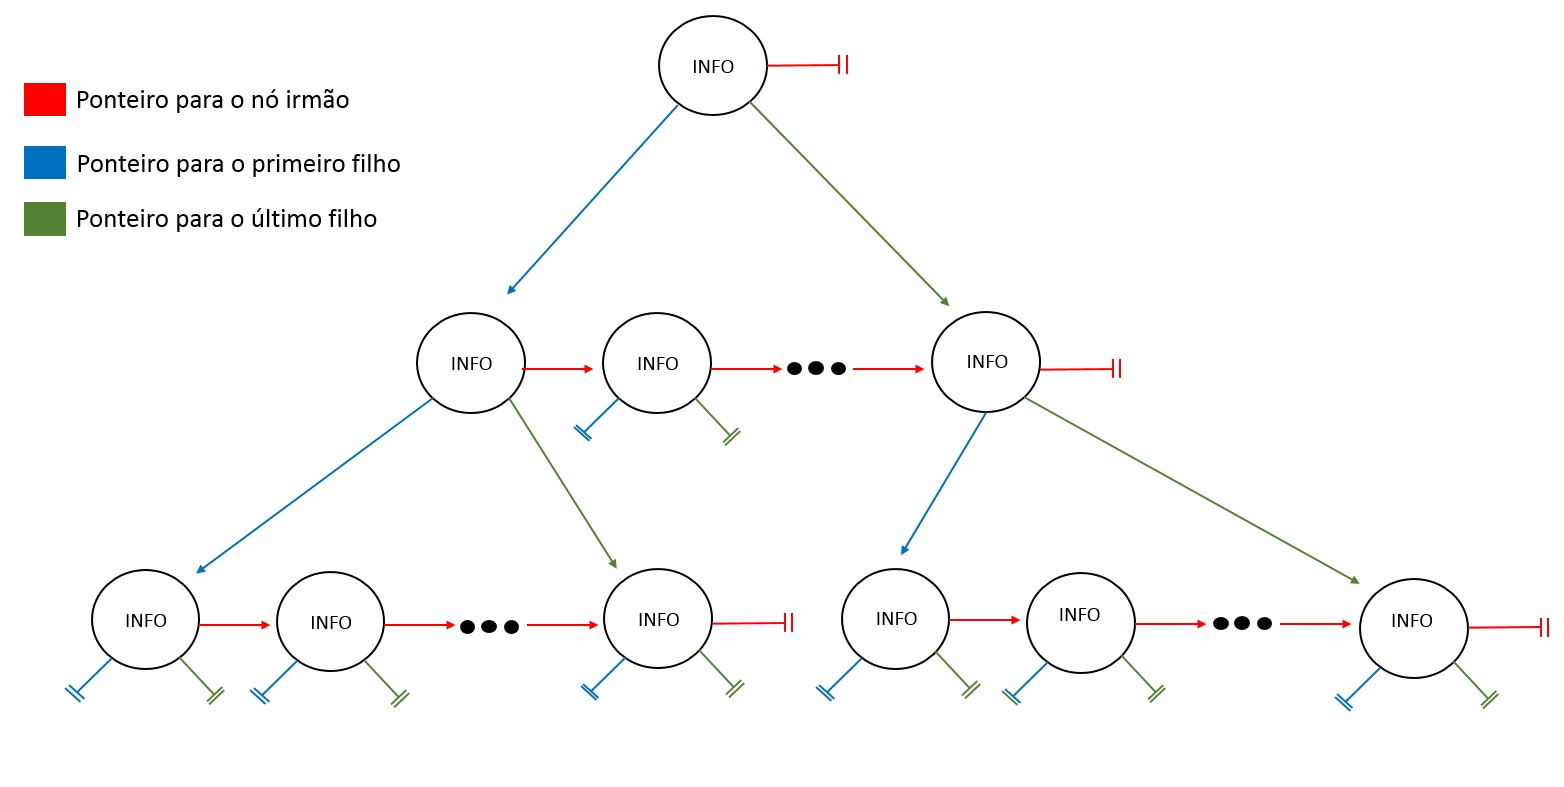
\includegraphics[width=160mm]{Arvore.jpg}
\caption{Diagrama do TAD árvore}
\label{fig:Tree} 
\end{figure}



\subsubsection{Manipulação da árvore}

\hspace{1.5em}Inicialmente, é criado a raíz da árvore, com a informação simbólica \emph{' \textbackslash0'}. 
A raíz da árvore possui uma lista de filhos que é formado pelos caracteres do axioma. A partir do axioma, 
é aplicado as regras contidas em \emph{rules}.

A aplicação das regras se baseia em percorrer as folhas da árvore, e para cada folha, verificar se sua informação 
é igual a algum \emph{p} da lista de regras \emph{rules}, se sim, inserir naquela folha uma lista de filhos onde cada nó contém um 
caracter da string \emph{s}. Este processo é repetido \emph{order} vezes.

Ao final de \emph{order} aplicações das regras, a string final é recolhida a partir de todas as folhas da árvore.



\subsection{Os comandos}

\hspace{1.5em}O desenvolvimento dos comandos foram divididos em duas etapas. A primeira é descrita na parte 1 do trabalho e a 
segunda etapa é descrita nas partes 2 e 3 do trabalho.


\subsubsection{Parte 1}

\hspace{1.5em}A string final, que é a concatenação das informações das folhas da árvore, é formada por qualquer caracter, podendo 
ser letras, números e símbolos, porém, para a primeira parte do trabalho, foi implementado apenas os comandos representados pelas letras 
F e G, e pelos símbolos +, -, [ e ].

Devido a possibilidade de haver símbolos ou caracteres indesejados além dos implementados, a string final é passada por um filtro eliminando-os.
Após o filtro, a string é impressa no arquivo de saída, junto ao preâmbulo.

Um exemplo de resultado obtido foi o triângulo de \emph{Sierpinski} na Figura \ref{fig:SierpinskiTriangle}, 
gerado a partir do seguinte \emph{grammar}:
\newpage
\begin{verbatim}
order 7
angle 3
axiom F

F = FXF
X = +FLXRF-FLXR<F-F>LXR<F+
L = >6
R = <6
\end{verbatim} 
\hspace{1.5em}A pesar de não ter sido implementado os comandos \emph{\textless} e \emph{\textgreater}, a figura ainda é gerada devido ao filtro 
que é aplicado à string final, porém em preto e branco.
\newline 
\begin{figure}[ht!]
\centering
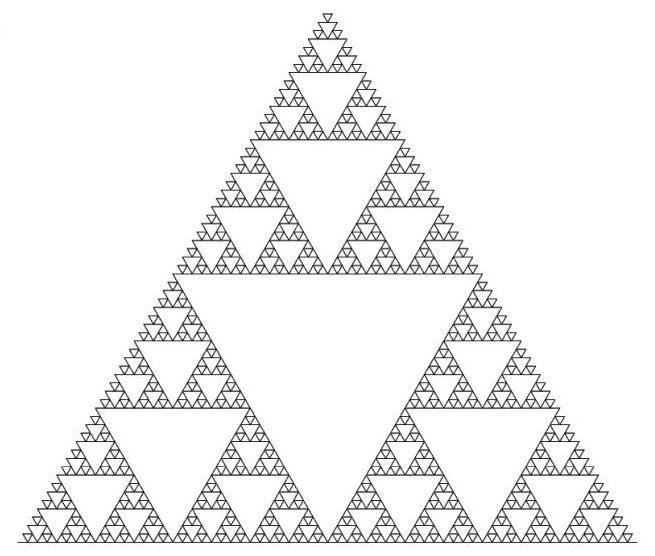
\includegraphics[width=120mm]{sierpinskitriangle.jpg}
\caption{Triângulo de Sierpinski}
\label{fig:SierpinskiTriangle} 
\end{figure}


Um outro exemplo de resultado obtido a partir do \emph{grammar} a seguir é a Figura \ref{fig:Sphinx}, que ficou indesejada, pois o comando \emph
{\textbar} não foi implementado para a primeira parte do trabalho, e como este comando realmente influencia como a imagem é gerada, ela ficou
desconfigurada em relação a desejada.
\newline
\begin{verbatim}
angle 6
order 5
axiom X

X = +FF-YFF+FF--FFF|X|F--YFFFYFFF|
Y = -FF+XFF-FF++FFF|Y|F++XFFFXFFF|
F = GG
G = G>G
\end{verbatim}


\begin{figure}[ht!]
\centering
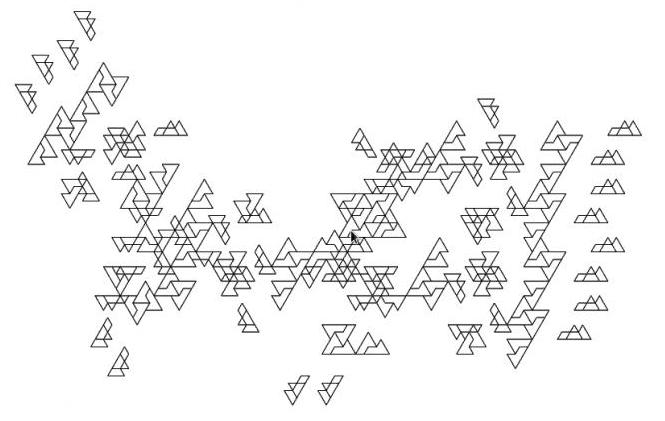
\includegraphics[width=120mm]{sphinx.jpg}
\caption{Sphinx (imagem indesejada)}
\label{fig:Sphinx} 
\end{figure}

Como para a primeira parte não foi implementado alguns comandos descritos no \emph{grammar}, a imagem não saiu como desejada, gerando 
apenas a resposta dos comandos que passaram pelo filtro.


\subsubsection{Partes 2 e 3}

\hspace{1.5em}Para a segunda e terceira parte, foi implementado uma estrutura de dados baseada no princípio \emph{LIFO}, que possui como
representação da informação a seguinte estrutura:
\newpage
\begin{verbatim}
typedef struct                    Estrutura Turtle. 
{
    double x;                     Posição x. 
    double y;                     Posição y. 
    double orientation;           Orientação (Ângulo). 
    double length;                Comprimento da linha. 
    int color;                    Cor da linha. 
    int counterclockwise;         Flag para sentido horário ou anti-horário. 
} Turtle;
\end{verbatim}

Esta estrutura, modela uma tartaruga, com sua posição atual, orientação, comprimento do passo, sentido em que ela gira e a cor que 
ela risca quando abaixa a caneta.

Antes de passar pelo último filtro, a string final gerada pela parte 1 é passada para a função \emph{secondPart()}, que é
interpretada caracter a caracter, gerando os comandos em postscript. Estes comandos são desenhados pela tartaruga, e são interpretados
de acordo com a lista a seguir:

\begin{itemize}
\item O comando \emph{F} é convertido para a string \emph{n x0 y0 m x1 y1 l s}, e a posição em \emph{Turtle} é atualizada.
\item O comando \emph{G} apenas atualiza a posição de \emph{Turtle}.
\item Os comandos \emph{+} e \emph{-} atualizam a orientaçao de \emph{Turtle}.
\item O comando \emph{[} salva a posição atual e todas as outras características de \emph{Turtle} naquele instante.
\item O comando \emph{]} recupera a última posição com as características desta posição e gera a string \emph{r g b setrgbcolor}, onde 
\emph{r}, \emph{g} e \emph{b} são os tons de vermelho, verde e azul da cor descrita no campo \emph{color} de \emph{Turtle}.
\item Os comandos \emph{\textless}, \emph{\textgreater} e \emph{c} atualizam a cor descrita no campo \emph{color} de \emph{Turtle}.
\item O comando \emph{@} atualiza o comprimento do passo da tartaruga, atualizando o campo \emph{length} de \emph{Turtle}.
\item O comando \emph{!} atualiza o sentido em que a tartaruga irá girar, atualizando o campo \emph{counterclockwise} de \emph{Turtle}.
\item O comando \emph{\textbar} gira a tartaruga 180 graus, atualizando o campo \emph{orientation} de \emph{Turtle}.
\end{itemize}

A implementação da cor se baseou em montar uma paleta de 256 cores, passando pelas cores marrom, verde, azul, anil, violeta, vermelho,
laranja, e voltanto ao marrom, em degradê. Para montar a paleta, foi utilizado como auxilio uma ferramenta disponível no site 
\url{www.strangeplanet.fr}\footnote{Para o link completo da paleta de cores gerada, ver Referência Bibliográfica \ref{GradientGenerator}}.

Um exemplo de resultado obtido foi a Sphinx na Figura \ref{fig:Sphinx2}, 
gerada a partir do seguinte \emph{grammar}:
\begin{verbatim}
angle 6
order 5
axiom X

X = +FF-YFF+FF--FFF|X|F--YFFFYFFF|
Y = -FF+XFF-FF++FFF|Y|F++XFFFXFFF|
F = GG
G = G>G
\end{verbatim} 
\hspace{1.5em}A Figura \ref{fig:Sphinx2} é a imagem desejada para a Figura \ref{fig:Sphinx}.
\newline 
\begin{figure}[ht!]
\centering
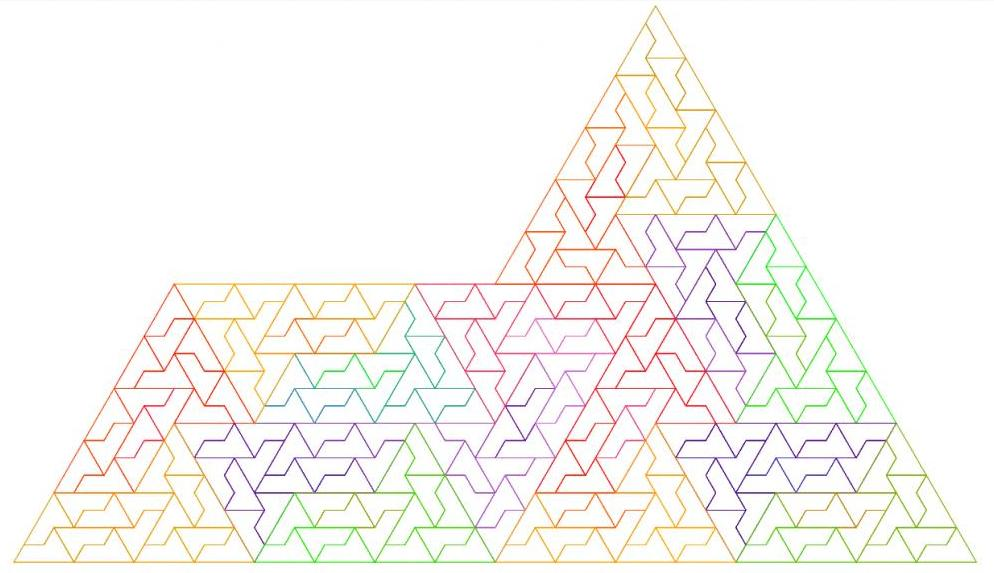
\includegraphics[width=140mm]{sphinx2.jpg}
\caption{Sphinx}
\label{fig:Sphinx2} 
\end{figure}

\newpage
%RESULTADOS E AVALIAÇÃO:
\section{Resultados e Avaliação}
\hspace{1.5em}Uma série de arquivos contendo os \emph{grammars} foram copiados do applet do \url{www.cgjennings.ca/toybox/lsystems/} para teste.

O resultado pode ser visto nos arquivos postscript que estão nas pastas \emph{Parte1-PS} e \emph{Parte2\&3-PS} que estão dentro da pasta 
\emph{Testes}.

A ferramenta valgrind foi frequentemente utilizada durante o desenvolvimento do sistema, 
sendo de grande ajuda para a depuração do programa.


%REFERÊNCIAS BIBLIOGRÁFICAS:
\section{Referências Bibliográficas}
\begin{enumerate}
\item Livro Introdução a Estrutura de Dados. Autores: Waldemar Celes, Renato Cerqueira e José Lucas Rangel.
\item \url{http://www.cgjennings.ca/toybox/lsystems/}
\item \url{http://algorithmicbotany.org/}
\item \label{GradientGenerator} \url{http://www.strangeplanet.fr/work/gradient-generator/?c=257:B8870B:00FF00:4169E1:4C0082:EE82EE:FF0000:FFA600:B8870B}
\item \url{http://www.mat.ufmg.br/~regi/topicos/intlat.pdf} 
\item \url{http://ctan.mirrorcatalogs.com/info/symbols/comprehensive/symbols-a4.pdf}
\item \url{http://tex.stackexchange.com} 
\end{enumerate}


\end{document}



